
\vspace{-5pt}
\subsection{Greedy Algorithms}

In this section, three simple greedy algorithms are presented. For brevity, consider only the valuation-maximizing problem ({\sc maxPA}). Furthermore, without loss of generality, assume $|S_k| \le C$ for all $k$. 

\begin{enumerate}

\item
{\em Greedy Valuation Algorithm} {\sc(GVA)}: First, sort customers in $\cN = \{1,...,n\}$ by their valuations in a non-increasing order (where ties are broken arbitrarily): \vspace{-5pt}
\begin{equation}
\mbox{if\ }  k \le k', \mbox{\ then\ }  
u_{k} \ge u_{k'}
\end{equation}
Then, select the demands in that order until the capacity constraint ($\big|\sum_{k\in {\cal N}}S_k x_k\big| \le C$) is not satisfied. 


\item 
{\em Greedy Demand Algorithm} {\sc(GDA)}: Similar to {\sc GVA}, but sort the customers by the magnitude of their demands in a non-decreasing order:  \vspace{-5pt}
\begin{equation}
\mbox{if\ }  k \le k', \mbox{\ then\ }  
|S_{k}| \le |S_{k'}|
\end{equation}
Then, select the demands in that order until the capacity constraint ($\big|\sum_{k\in {\cal N}}S_k x_k\big| \le C$) is not satisfied. 

\item 
{\em Greedy Ratio Algorithm} {\sc (GRA)}: Similar to {\sc GVA} and {\sc GDA}, but sort the customers by the efficiency ($\frac{u_k}{|S_k|}$) in a non-increasing order:  %\vspace{-5pt}
\begin{equation}
\mbox{if\ }  k \le k', \mbox{\ then\ }  
\frac{u_k}{|S_k|} \ge \frac{u_{k'}}{|S_{k'}|} 
\end{equation}
Then, select the greedy solution $X$ in that order until the capacity constraint ($\big|\sum_{k\in X}S_k x_k\big| \le C$) is not satisfied. Lastly, return the maximum valuation of two candidate solutions: either greedy solution $X$, or the maximum valuation of a single customer $\arg\max_{k\in \cN}\{ u_k\}$. Fig.~\ref{fig:alge} presents a flowchart of {\sc GRA}.
\end{enumerate}

%\begin{algorithm}[htb!]
%\caption{${\sc GRA} [ \{u_k,S_k(t)\}_{k \in \cN}, C]$}
%\begin{algorithmic}[1]
%\Require customers' utilities and demands $\{u_k,S_k(t)\}_{k\in \cN}$; capacity $C$
%\Ensure $(\frac{1}{2} \sqrt{\frac{\cos \theta + 1}{2}},1)$-solution $\hat{S}$ to \textsc{CKP}
%\State Sort customers in $\cN$ by their efficiency defined by Eqn.~\raf{eq:ef}
%\State $S_1 \leftarrow \varnothing$
%\For{$k \in \cN$} 
%\If{ $\big|\sum_{k' \in S_1} d_{k'} + S_k(t) \big| \le C$} \label{alg:g.feas}
%\State $S_1 \leftarrow S_1 \cup \{k\}$ \label{alg:g.add}
%\EndIf
%\EndFor
%\State Set $S_2 \leftarrow \{\displaystyle {\arg\max}_{k \in \cN   } u_k \}$
%\State Set $\hat{S} \leftarrow \arg\max_{S_1, S_2}\{ u(S_1), u(S_2) \}$ \label{alg:g.max}
%\State \Return $\hat{S}$
%\end{algorithmic}
%\end{algorithm}

\begin{figure}[!ht]
\centering\vspace{-5pt} 
 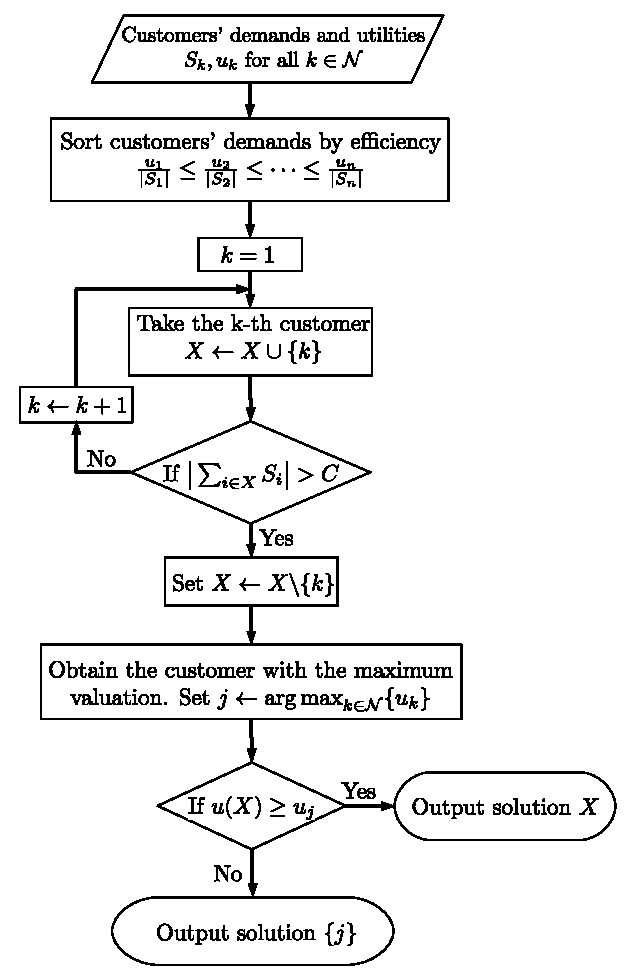
\includegraphics[scale=0.6]{fig/flow-chart-greedy-e.pdf}
\caption{Flow chart for Greedy Ratio Algorithm {\sc (GRA)}.} \vspace{-5pt} 
\label{fig:alge}
\end{figure}

{\sc GVA} and {\sc GDA} are common strategies of load curtailment in practice. 
However, {\sc GRA} possesses a worst-case guarantee, and shows a good empirical ratio with the optimal solutions in simulations.
\\

\begin{customthm}{1} \label{thm:alg-greedy}
Algorithm {\sc GRA} produces a feasible solution within a worst-case guarantee of $\frac{1}{2} \sqrt{\frac{\cos \theta + 1}{2}}$ of the optimal solution of \textsc{maxPA}.
\end{customthm}
\

The worst-case guarantee of {\sc GRA} depends on $\theta$; the smaller the $\theta$, the better guarantee it provides. The basic idea of the proof is discussed in the Appendix. Algorithm {\sc GRA} can be applied to {\sc minPA} by defining the efficiency as ($\frac{c_k}{|S_k|}$). For {\sc minPA}, the worst-case guarantee does not apply, but still shows a good empirical ratio to the optimal solutions by simulations.
